\chapter {Introduction}

\section{Problem Statement}

% \subsection{Sub-Section Title (Layer 3)}

Implicit biases introduced by the optimization algorithm play a crucial role in deep learning and in the generalization ability of the learned models. In particular, minimizing the training error, without explicit regularization, over models with more parameters and capacity than the number of training examples, often yields good generalization.

Do we still benefit from implicit regularization when minimizing the logistic loss on separable data? While it is clear that the norm of the predictor itself is not minimized, since it grows to infinity, for prediction, only the direction of the predictor, i.e. the normalized $w(t)/ ||w(t)||$ , is important. How does $w(t)/ ||w(t)||$ behave as $t \rightarrow +\infty$ when we minimize the logistic (or similar) loss using gradient descent on separable data, i.e., when it is possible to get zero misclassification error and thus drive the loss to zero?

Overall, implicit bias in gradient descent can have significant negative consequences, particularly when it leads to unfair or discriminatory outcomes. It's important for machine learning practitioners to be aware of these issues and take steps to address them, such as by using diverse training data, testing for biases in the data, and using debiasing algorithms.

\chapter{Related Work}

\section{Problem Statement}

The paper we selected for the research, “The Implicit Bias of Gradient Descent on Separable Data”, introduced various methods of gradient descent and compared the implicit biases between each of the models to show the accuracy of their results.

In this paper, the authors examine gradient descent on unregularized logistic regression problems, with homogeneous linear predictors on linearly separable datasets. We show the predictor converges to the direction of the max-margin (hard margin SVM) solution. The result also generalizes to other monotone decreasing loss functions with an infimum at infinity, to multi-class problems, and to training a weight layer in a deep network in a certain restricted setting. Furthermore, we show this convergence is very slow, and only logarithmic in the convergence of the loss itself. This can help explain the benefit of continuing to optimize the logistic or cross-entropy loss even after the training error is zero and the training loss is extremely small, and, as we show, even if the validation loss increases. Our methodology can also aid in understanding implicit regularization in more complex models and with other optimization methods.

\section{Novelty}

For our research, we intend to implement another gradient algorithm that we had learned from the class, and compare its results to determine the implicit biases between the gradient descent algorithms. Our objective is to minimize the validation error of the data by providing a more lenient tolerance of the training error.

\chapter{Methods}

\section{Algorithm}

\subsection{Gradient Descent}

\subsection{Gradient Descent}

\subsection{Gradient Descent}

\section{Dataset}

\chapter{Evaluation}
\section{Gradient Descent}
Firstly, we implemented the original code from the paper, and got the training results. Below are the rate of training precision and validating precision, for training 80 epochs.

\begin{figure}[h]
    \centering % figure is centered on the page
        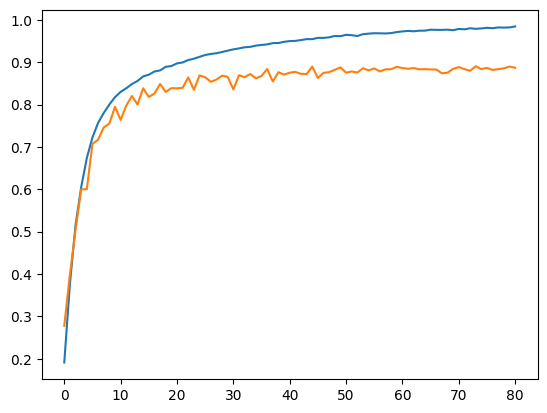
\includegraphics[width=0.8\linewidth]{./output.png} 
    \caption{Training precision and validating precision.}
    \label{figure:sample figure} % assign a unique label to each figure
\end{figure}

% \begin{table}[h]
%     \centering % table is centered on the page
%     \caption{This is how you make a table.} % The caption of the table is defined here
%     \label{table:sample table} % Assign a unique label to each table
%     \begin{tabular}{llcr} 
%         \toprule
%             & \textbf{parameter} & \textbf{type 1} & \textbf{type 2}\\
%         \midrule
%             $k_{0}$  & something     & $x$           & $y$\\
%             $k_{0}$  & other thing   & $E = mc^2$    & $z$\\ 
%             $\tau$   & exponent      & 2             & 3 \\
%         \bottomrule
%     \end{tabular}
% \end{table}



\section{Gradient Descent}

\section{Gradient Descent}

\chapter{Conclusion}

\chapter{Acknowledgements}

\chapter{Reference}